\documentclass[tikz]{standalone}

\begin{document}
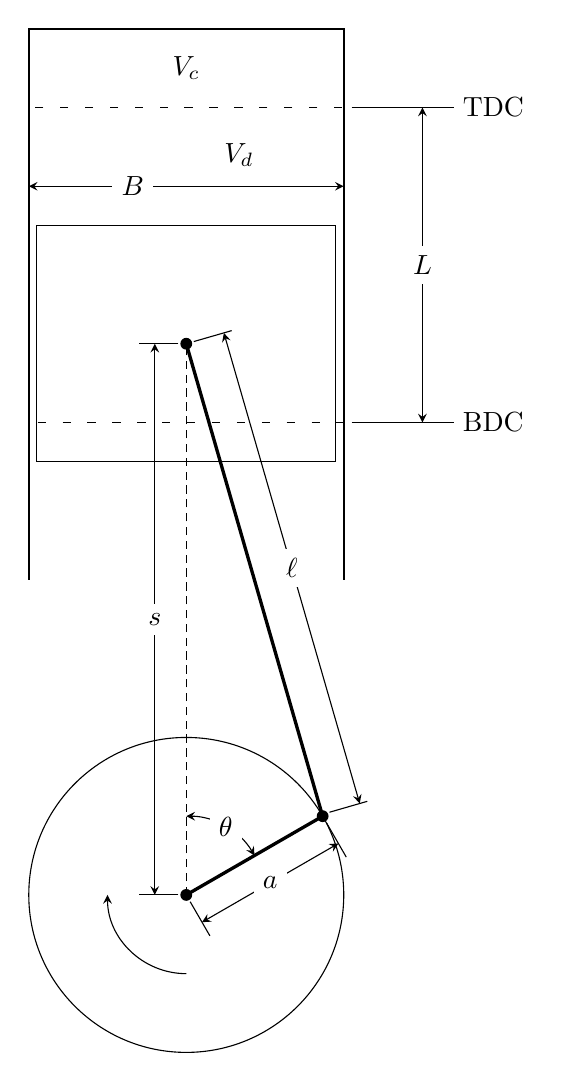
\begin{tikzpicture}
%Crank
\draw (0,0) circle (2);
\fill[black] (0,0) circle (0.075);
%Crank rod
\draw[very thick] (0,0) -- (30:2) -- (0,7);
%Cylinder wall
\draw[thick] (-2,4) -- ++(0,7) -- ++(4,0) -- ++(0,-7);
%Piston
\draw (-1.9,5.5) -- ++(0,3) -- ++(3.8,0) -- ++(0,-3) -- cycle;
\fill[black] (0,0) (30:2) circle (0.075);
\fill[black] (0,7) circle (0.075);
\draw[densely dashed] (0,0) -- (0,7);
\draw[loosely dashed] (-2,10) rectangle (2,6);
\draw (2.1,10) -- ++(1.3,0) node at +(0.5,0) {TDC};
\draw (2.1,6) -- ++(1.3,0) node at +(0.5,0) {BDC};
\draw[stealth-stealth] (3,10) -- (3,6) node[fill=white] at +(0,2) {$L$};
\draw (-0.1,7) -- ++(-0.5,0);
\draw (-0.1,0) -- ++(-0.5,0);
\draw[stealth-stealth] (-0.4,0) -- ++(0,7) node[fill=white] at +(0,-3.5) {$s$};
\draw[stealth-stealth] (0,1) arc(90:30:1) node[fill=white] at (60:1) {$\theta$};
\draw (-60:0.1) -- ++(-60:0.5);
\draw (30:2) ++(-60:0.1) -- ++(-60:0.5);
\draw[stealth-stealth] (-60:0.4) -- ++(30:2) node[fill=white,midway] {$a$};
\draw (30:2.1) -- ++(16.1021:0.5);
\draw (0,7) ++(16.1021:0.1) -- ++(16.1021:0.5);
\draw[stealth-stealth] (30:2.1) ++(16.1021:0.4) -- ++(106.1021:6.22) node[fill=white,midway] {$\ell$};
\draw[-stealth] (-90:1) arc(-90:-180:1);
\node at (0,10.5) {$V_c$};
\node at (0.67,9.4) {$V_d$};
\draw[stealth-stealth] (-2,9) -- ++(4,0) node[fill=white,pos=0.33] {$B$};
\end{tikzpicture}
\end{document}